\chapter{Introduction}

Telecommunications engineering plays a key role in the development of technologies based on electronics, instrumentation and advanced signal processing. One of the emerging fields where these disciplines converge is biomedical engineering, specifically in the analysis and processing of physiological signals for rehabilitation and prosthetic control applications.

Specifically, the study of signals such as electromyography (EMG) makes it possible to obtain detailed information about muscular activity, which is essential for understanding the neuromuscular system and designing assistive devices. The correct interpretation of these signals depends not only on accurate data acquisition, but also on the use of advanced processing techniques, including feature extraction and source separation algorithms.

Additionally, signal separation is a commonly applied tool in the field of telecommunications, especially given the relevance of wireless communications and 
radio systems. In these technologies, multiple transmitters may broadcast signals at nearby frequencies, causing them to overlap with one another and with other sources of interference. As a result, it is necessary to separate these signals in order to recover the desired information and monitor the spectrum effectively. 
\\
\begin{figure}[H]
    \centering
    \makebox[\textwidth][c]{%
        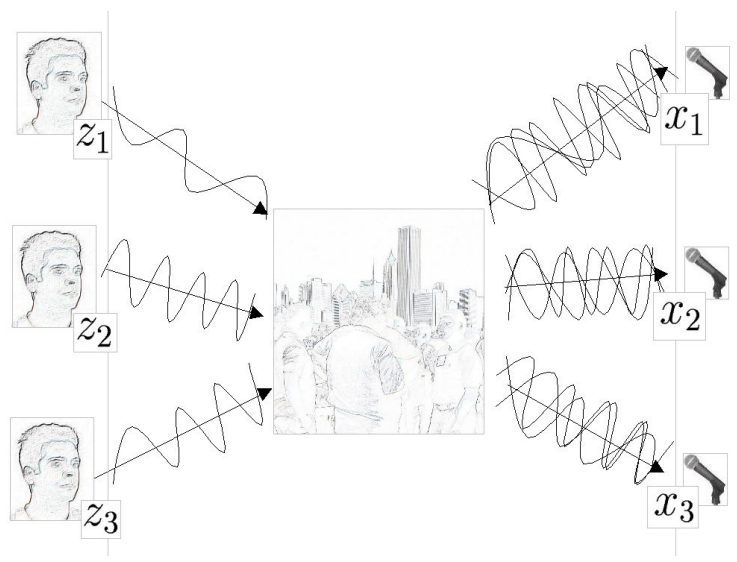
\includegraphics[width=\linewidth, height=5cm]{figuras/cocktail_party.png}
    }
    \caption{Typical example of the cocktail party. Independent speakers are superimposed and recorded by three independent microphones. Figure was extracted from \texttt{Biomedical Signal and Image Processing} \cite{clifford_biomedical_2008}.}
    \label{fig:cocktail_party}
\end{figure}
Although these applications mainly belong to the field of telecommunications, they contain valuable concepts that can also be applied to biomedical signals such as EMG. This Bachelor’s Thesis focuses on the development of separation algorithms for EMG signals, with the aim of improving the quality of the processed signals and facilitating their use in clinical and research environments.

\section{Background and context}

This thesis is closely related to a research project developed at the Institute for Research in Technology of Comillas Pontifical University, commonly known by its Spanish acronym IIT (\textit{Instituto de Investigación Tecnológica}). In particular, it is inspired by the project on implantable EMG systems for myoelectric orthoses and bionic reconstruction after severe peripheral nerve injuries \cite{giannetti_ortesis_nodate}.

The project focuses on implantable and wireless myoelectric signal acquisition systems intended for the control of exoskeleton orthoses. These systems belong to the field of human-machine interfaces, where physiological signals such as EMG are used to estimate the user's motor intention and translate it into control commands for devices.

\begin{figure}[H]
    \centering
    \makebox[\textwidth][c]{%
        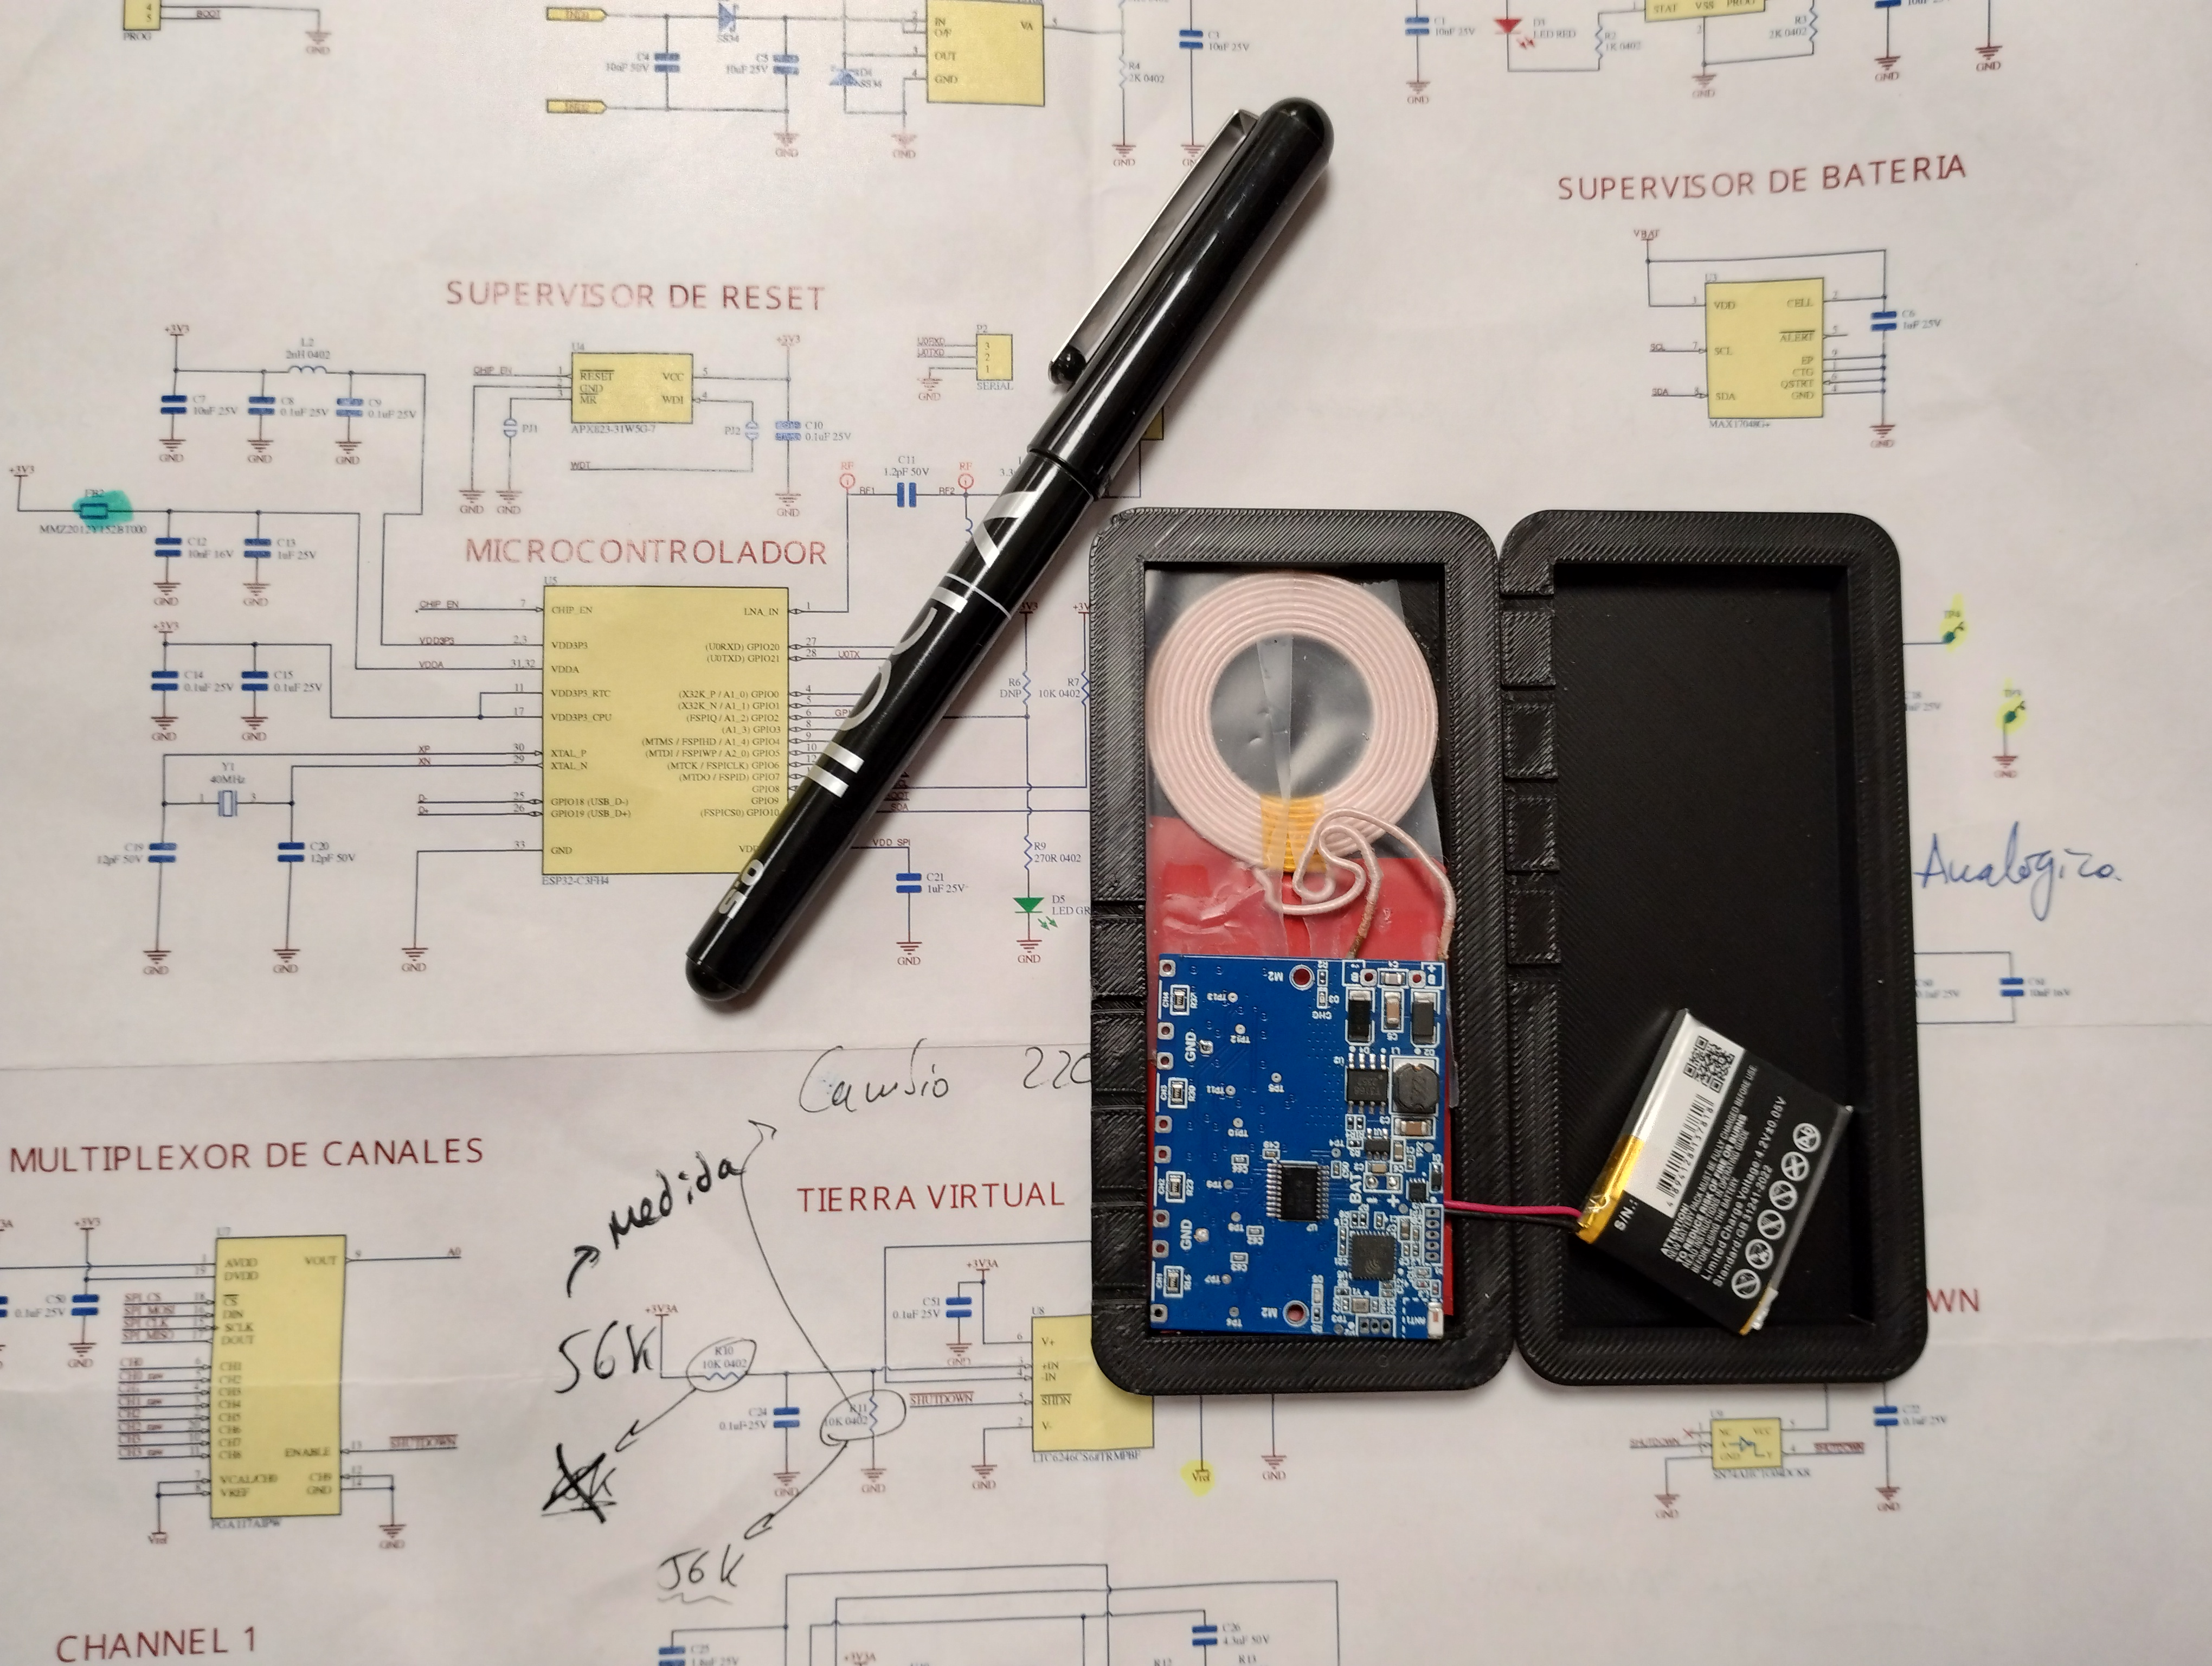
\includegraphics[width=\linewidth, height=6cm ]{figuras/iit_schematics.jpg}
    }
    \caption{Prototype (v2) of a wireless, Bluetooth Low Energy EMG sensor, designed to be long term implanted by the authors of \cite{giannetti_ortesis_nodate}.}
    \label{fig:iit_schematics}
\end{figure}
In this context, EMG signals provide a direct measurement of muscular activation and are therefore widely used in prosthetic and orthotic control. However, their practical use depends strongly on the quality and stability of the recorded signals, especially when these signals are obtained from reinnervated muscles.


\section{Motivation}
\label{sec:motivation}



Peripheral nerve injuries and limb loss can drastically affect motor function, sensitivity and the ability to perform daily activities. Although reconstructive surgery has advanced significantly over the past few years, functional recovery is not always sufficient to restore natural control of the affected limb. For this reason, myoelectric prostheses have become an important technological alternative, as they use EMG signals to infer the user's motor intention and translate it into control commands.

When a limb is amputated, the motor nerves at the end of the residual limb are sectioned. If they are not reconnected to a functional biological structure, they may form disorganized and painful nerve endings. To improve neuromuscular integration and provide more reliable control signals, several surgical strategies have been proposed. One of the most established techniques is Targeted Muscle Reinnervation (TMR), where motor nerves are redirected to reinnervate residual muscles that no longer serve their original function. These muscles then act as biological amplifiers of the neural commands, generating EMG activity that can be detected and used for prosthetic control.

\begin{figure}[H]
    \centering
    \begin{subfigure}[b]{0.4\textwidth}
        \centering
        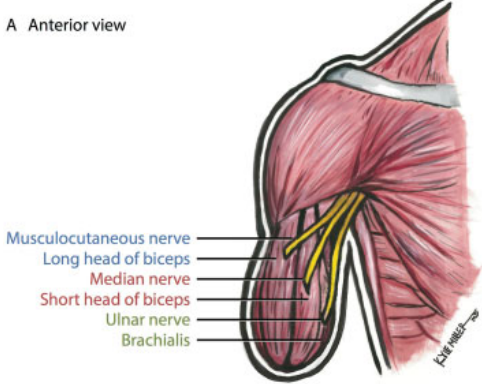
\includegraphics[width=\textwidth, height=0.93\textwidth]{latex/anexos/Anexo B/figuras/TMR_anterior.png}
        \caption{Anterior view}
        \label{fig:2a}
    \end{subfigure}
    \hfill
    \begin{subfigure}[b]{0.45\textwidth}
        \centering
        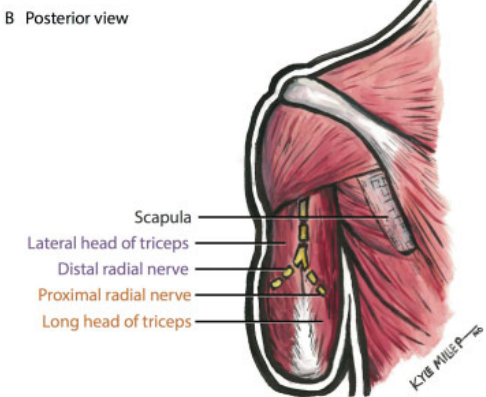
\includegraphics[width=\textwidth]{latex/anexos/Anexo B/figuras/TMR_posterior.png}
        \caption{Posterior view}
        \label{fig:2b}
    \end{subfigure}
    \caption{Schematic representation of the surgical plan for TMR in transhumeral amputation \cite{cheesborough_targeted_2015}. Labels of the same color represent the muscles and their innervation origin.}
    \label{fig:comparison_TMR}
\end{figure}

Additionally, Regenerative Peripheral Nerve Interfaces (RPNIs) consist of implanting a free denervated muscle graft directly onto the affected nerve, creating a localized biological amplifier that can generate high-quality EMG signals with reduced contamination from nearby muscles \cite{pettersen_regenerative_nodate}. More recently, Vascularized Denervated Muscle Targets (VDMTs) have also been explored as an alternative interface, combining the idea of a denervated muscle target with vascularized tissue to improve long-term viability and signal quality \cite{gonzalez-prieto_regenerative_2024,v_use_2022}.

\begin{figure}[H]
    \centering
    \makebox[\textwidth][c]{%
        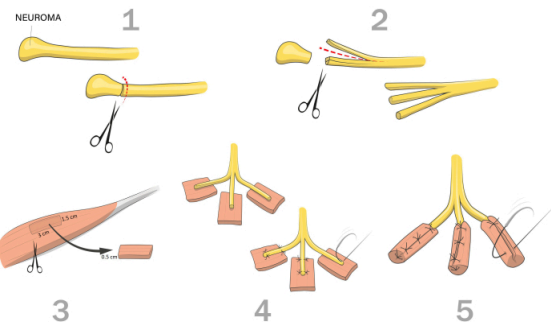
\includegraphics[width=\linewidth, height=4.5cm ]{figuras/RPNI_procedure.png}
    }
    \caption{Illustration of the Regenerative Peripheral Nerve Interface (RPNI) procedure \cite{pettersen_regenerative_nodate}.}
    \label{fig:RPNI_procedure}
\end{figure}

However, although these techniques improve the quality and acquisition of control signals, they also introduce new signal processing challenges. When auxiliary muscles are used as biological amplifiers, the redirected nerve interacts with a new muscular environment. This can modify the morphology, amplitude and temporal structure of the recorded EMG signal. Changes in the geometry and density of motor unit sources affect how the motor unit action potentials propagate through tissue, leading to signals that may differ significantly from those recorded in healthy muscles.

As a result, EMG recordings in these contexts may present amplitude attenuation, temporal delays, atypical activation patterns and contamination from adjacent muscular sources. These effects can make the desired information difficult to identify, especially when the target component is weak compared to other dominant sources. This is particularly relevant for prosthetic control, where inaccurate detection of muscular activation can reduce quality of responses and reliability.

\begin{figure}[H]
    \centering
    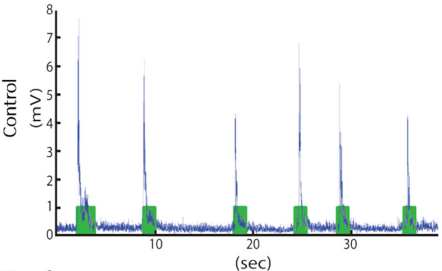
\includegraphics[width=0.8\linewidth,height=5.5cm]{latex/anexos/Anexo B/figuras/RPNI_Control.png}
    \caption{Native muscle EMG activity during a 40 second recording \cite{frost_regenerative_2018}. Activation patterns identified by algorithms.}
    \label{fig:RPNI_C}
\end{figure}

\begin{figure}[H]
    \centering
    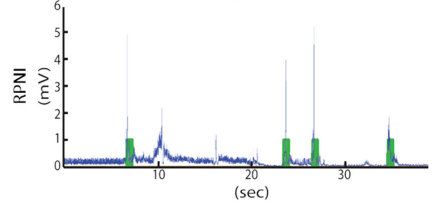
\includegraphics[width=0.8\linewidth,height=6cm]{latex/anexos/Anexo B/figuras/RPNI.png}
    \caption{EMG activity recorded from the RPNI during a 40 second trial \cite{frost_regenerative_2018}. Activation patterns are irregular and delayed, which makes it harder for EMG prosthetic control.}
    \label{fig:RPNI_O}
\end{figure}
\clearpage
Therefore, the motivation of this Bachelor's Thesis is to study whether signal separation techniques can help recover weak EMG components from mixed recordings. By identifying and separating the target activity from stronger interfering components, the objective is to improve the quality of the processed EMG signals, ultimately contributing to more reliable EMG control strategies for prosthetic applications.

\section{Problem statement}

VDMTs help prevent the reinnervated muscle from atrophying by maintaining a vascularized muscular environment. However, this configuration can also introduce significant interference from the donor muscle when measuring the EMG activity associated with the reinnervated target. As a result, the recorded signal may contain a weak component of interest superimposed with a stronger contribution from the surrounding donor muscle.

Although this thesis studies EMG signal separation under several possible conditions, its main motivation is the interference problem introduced by the IIT project. For this reason, the work focuses on separating a weak reinnervated-muscle signal from stronger donor muscle interference under controlled mixing conditions.

To achieve this, several obstacles must be considered, including source dominance, additive noise and possible temporal delays between channels. These factors are especially relevant because they determine whether each separation method can recover the target activity reliably or whether the weak component remains masked by the interfering source.
\begin{figure}[H]
    \centering
    \makebox[\textwidth][c]{%
        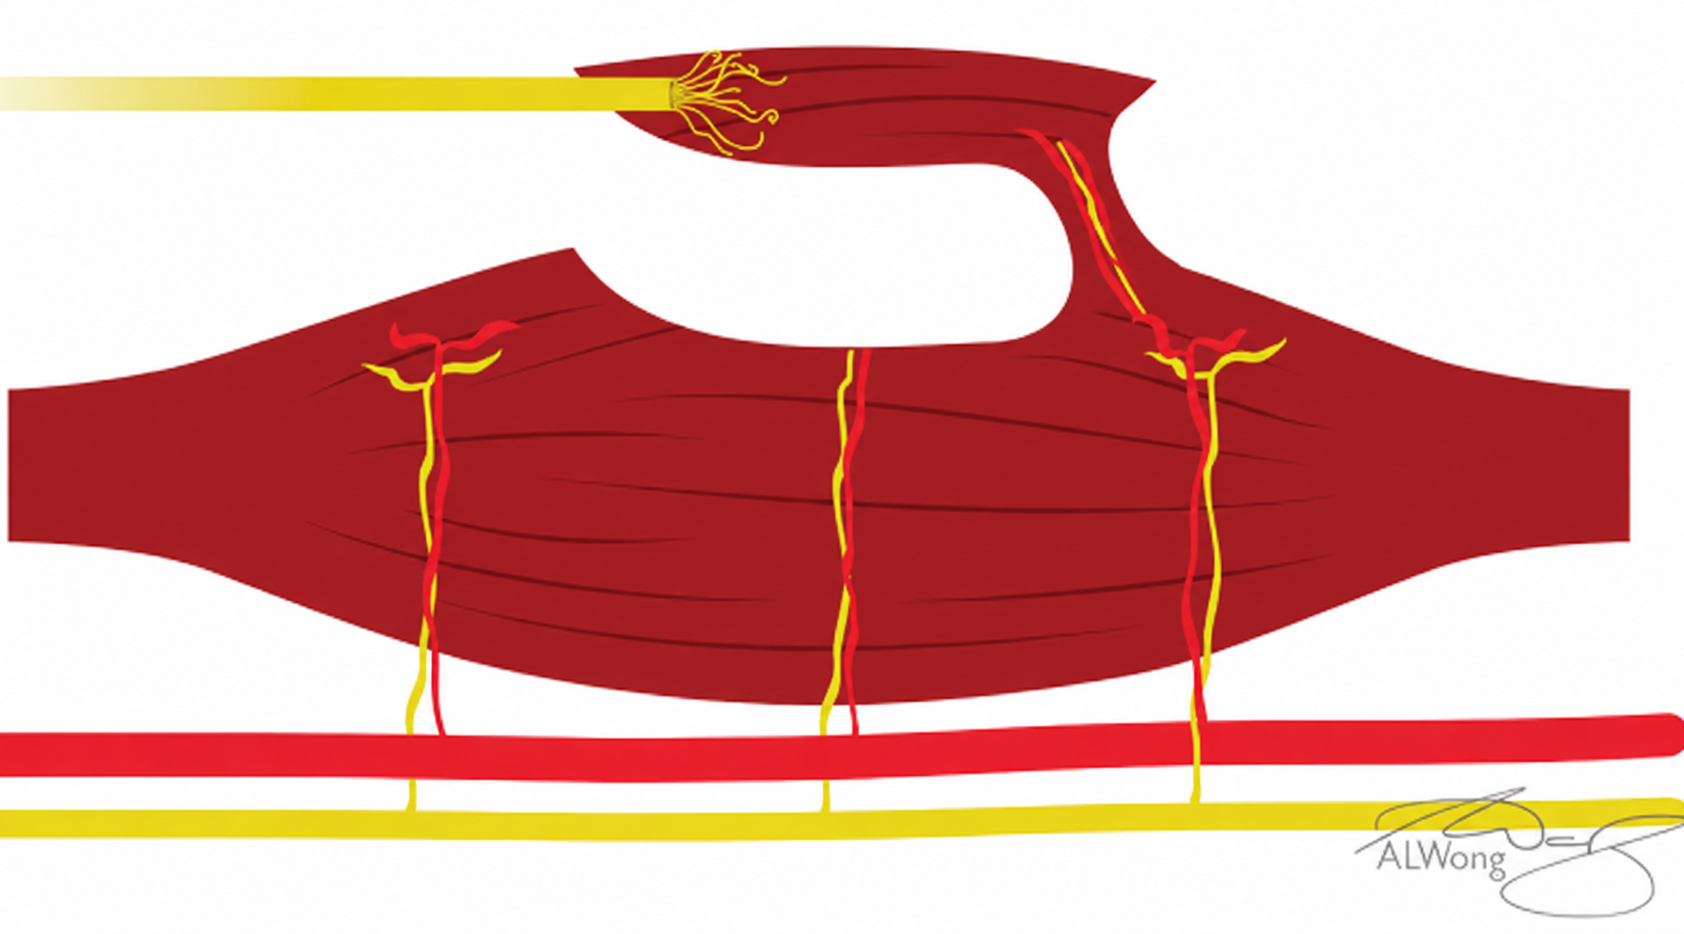
\includegraphics[width=\linewidth, height=6.5cm ]{figuras/VDMT_diagram_modified.png}
    }
    \caption{Adapted schematic illustration of a VDMT \cite{tuffaha_vascularized_2020}. The connection between the reinnervated muscle and the vascularized donor tissue motivates the interference problem addressed in this thesis.} 
    \label{fig:VDMT_diagram}
\end{figure}
\clearpage
\section{Objectives}
\label{sec:Objectives}

The main objective of this thesis is to evaluate source separation strategies for recovering weak EMG components in reinnervated muscle scenarios affected by donor-muscle interference.

To achieve this goal, the following specific objectives are proposed:

\begin{itemize}
    \item Analyze EMG signals generated by reinnervated muscles.
    \item Design a preprocessing pipeline to prepare EMG signals for the separation process.
    \item Discuss different source separation algorithms and study their performance under realistic scenarios.
    
    \item Assess whether instantaneous separation models can efficiently separate sources in the presence of small delays and additive noise.
    \item Evaluate whether including physiological information can improve the separation process.
    \item Assess whether the proposed algorithms can be implemented in real time.
\end{itemize}
